\subsection{One Lepton background}
\label{sec:bkgOL}

%In this analysis, the SM backgrounds with one real lepton in the final state come from W decays, either through direct W production or W boson��s 
In this analysis, the SM backgrounds with one real lepton in the final state come from W decays, either through direct W production of W bosons
from top decays.  The neutrino from the W decay is the source of real \MET, potentially smeared out due to resolution effects.
%
Given our baseline requirements of \MET $\ge $ 250\GeV and \MT$\ge$ 150\GeV, this background is dominated by direct W production.
We can thus estimate it by extrapolating from zero b-tag control regions. 
For MT2W$\ge $ 200 GeV, we choose two such regions, both with \MET$\ge$ 250\GeV, one for exactly 3 jets, and one for $\ge$ 4 jets.
For MT2W$<$ 200 GeV, even a potential zero b-tag control region would be dominated by lost lepton background. 
Furthermore, the one lepton background accounts for
less than 10\% of the total background for MT2W$<$ 200\GeV, and a data driven estimate is thus not warranted.
%
Similarily, the one lepton background from ttbar is a sufficiently small fraction of the total background that
it does not warrant a data driven estimate.

In the following, we first describe in detail the data driven estimate for the W jets background, including its systematic error, and then
conclude with Tables of the total one lepton background, including the parts taken from simulation. Additional details on the latter are provided
in the Appendix. The Appendix also includes crosschecks in data to further justify the conclusion that one lepton background from W's from top
decay is always small compared to other sources of background.
  
\subsubsection{Estimation Method from Data}
\label{subsec:bkg1L:Data}

Our control region to signal region extrapolation for the W plus jets background is based on the following assumption:

\begin{equation}\label{eq:btag_CR_ratios}
\frac{N^{data}_{0-btag}}{N^{data}_{\ge1-btag}} = \frac{N^{MC}_{0-btag}}{N^{MC}_{\ge1-btag}}
\end{equation}

Eq. ~\ref{eq:btag_CR_ratios} allows us to use normalize the background estimate in data in a 0-btag region, and then use simulation
to extrapolate from there to the corresponding $\ge$ 1 b-tag signal region as follows:
%
\begin{equation}\label{eq:btag_CR_ratios2}
N^{W+Jets}_{SR,\ge1-btag} = N^{data,WJets}_{CR,0-btag} \times \frac{N^{MC,WJets}_{SR,\ge1-btag}}{N^{MC,WJets}_{CR,0-btag}}
\end{equation}
%
Here $N^{data,WJets}_{SR,\ge 1-btag}$ is the estimated W+Jets contribution to each SR, 
$N^{data,WJets}_{0-btag}$ is the number of W+Jets events according to data in the CR, 
and ${N^{MC,WJets}_{\ge1-btag}}{N^{MC,WJets}_{0-btag}}$ is the 0-btag to 1-btag extrapolation factor.  
To obtain $N^{data,WJets}_{0-btag}$, we take the total data yield in the CR and subtract the 
non-WJets contribution according to MC prediction:
\begin{equation}\label{eq:wjetsyield}
N^{data,WJets}_{CR,0-btag} = N^{data}_{CR,0-btag} - N^{non-WJets MC}_{CR,0-btag}
\end{equation}

In practice, we do not have sufficient statistics in the zero b-tag sample to form a dedicated CR for every SR.
As a compromise between statistical and systematic error, we define two such W+jets CRs as follows:
\begin{itemize}
\item CR1:  0-btags, \MET $>$ 250 GeV, exactly 3 jets to estimate W+Jets for the 3 jet SRs.
\item CR2:  0-btags, \MET $>$ 250 GeV, $\ge$ 4 jets to estimate W+Jets for the $\ge$ 4 jets SRs.
\end{itemize}
This implies that we employ a second extrapolation in \MET from our inclusive \MET$\ge$ 250 \GeV baseline region to
the various exclusive \MET bins. 

We define the two aforementioned extrapolation factors as follows:
%
\begin{equation}\label{eq:tfmet}
TF_{MET}(\MET, njets) = \frac{N^{MC,WJets}_{0-btag}(\MET,njets)}{N^{MC,WJets}_{0-btag,\MET>250}(njets)}
\end{equation}
%
\begin{equation}\label{eq:tfbtag}
TF_{btag}(\MET, njets) = \frac{N^{MC,WJets}_{\ge1-btag,SR}(\MET,njets)}{N^{MC,WJets}_{0-btag,CR}(\MET,njets)}
\end{equation}
%
$TF_{MET}$ extrapolates only in \MET at fixed jet multiplicity and for the zero b-tag distributions, while
$TF_{btag}$ extrapolates only in the number of b-tags at fixed \MET and fixed jet multiplicity.

\subsubsection{Data versus MC Crosschecks of the \MET distribution}\label{subsec:METStudy}

{\bf fkw comments: I don't see why we keep this in the main text. I would put this into the appendix as it is in no way used to derive the actual background estimate.}

As discussed in Section~\ref{sec:bkgOL}, we use the simulation to extrapolate in \MET from an inclusive region \MET $\ge$ 250 \GeV into
into multiple inclusive \MET bins. In the present section we provide several data vs MC comparison of \MET distributions in 
zero b-tag control regions as crosschecks for this extrapolation.
These W+Jets CRs are summarized in Table~\ref{tab:WJetsCRsMET} and the corresponding \MET distributions are shown in Figures~\ref{fig:METDist}. 

\begin{figure}[h]
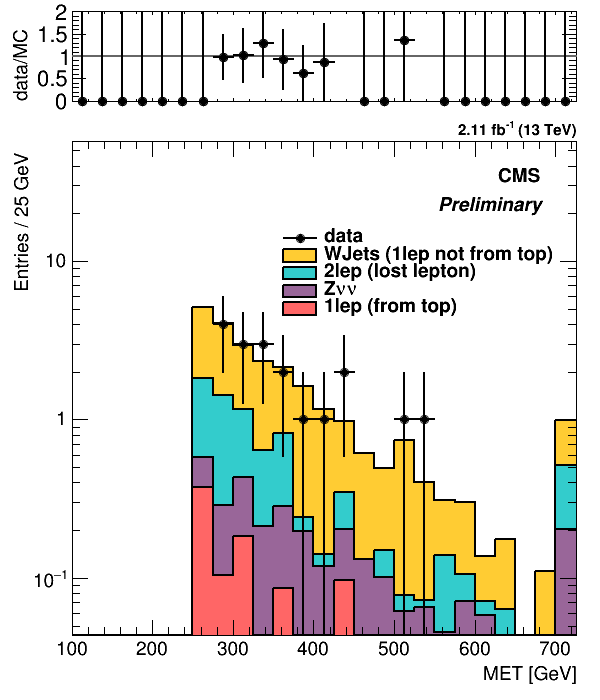
\includegraphics[width=0.44\textwidth]{Figures/bkg1lep/MET_MET250_MT120_4jets.png}
%\includegraphics[width=0.32\textwidth]{Figures/bkg1lep/MET_MET250_MTband_4jets.png}
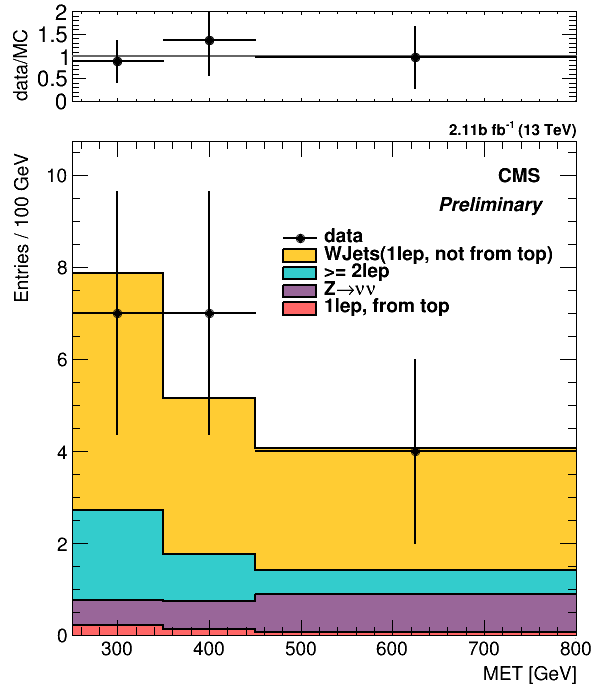
\includegraphics[width=0.44\textwidth]{Figures/bkg1lep/MET_MET250_MT150_4jets.png}
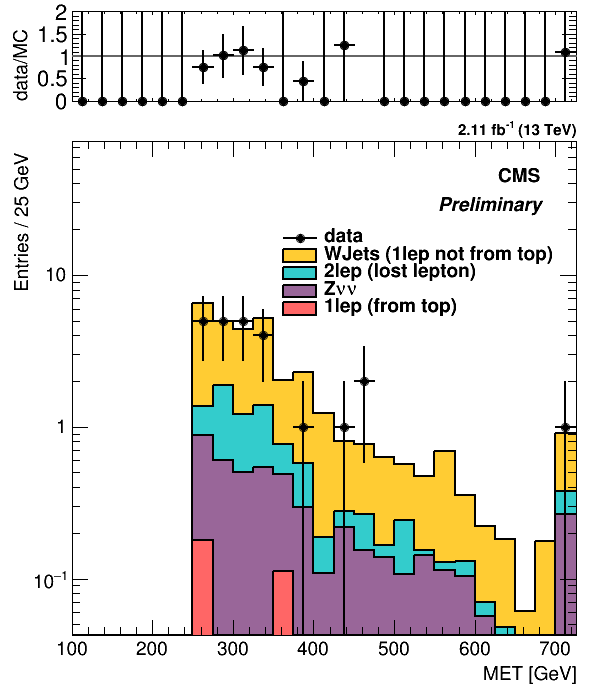
\includegraphics[width=0.44\textwidth]{Figures/bkg1lep/MET_MET250_MT120_3jets.png}
%\includegraphics[width=0.32\textwidth]{Figures/bkg1lep/MET_MET250_MTband_3jets.png}
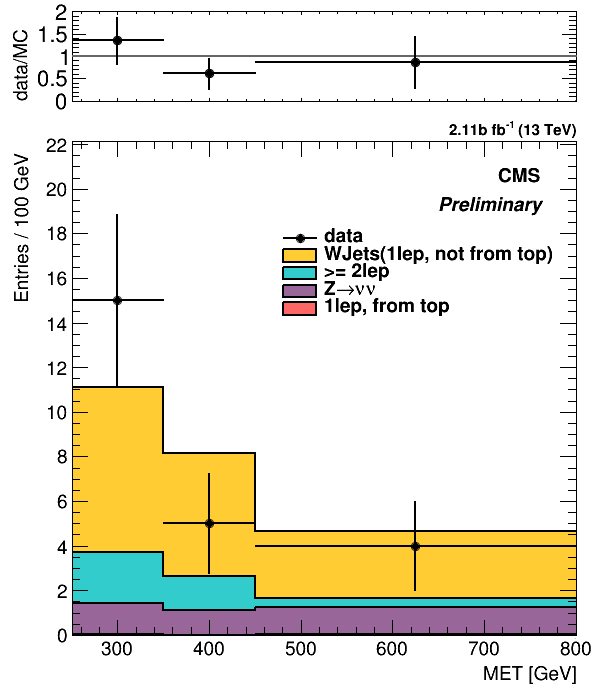
\includegraphics[width=0.44\textwidth]{Figures/bkg1lep/MET_MET250_MT150_3jets.png}
\caption{\label{fig:METDist} Distribution of \MET in different 0-btag,  3 and $\ge$ 4 jets CRs.}
\end{figure}


\begin{table}
\begin{center}
\small
\caption{\label{tab:WJetsCRsMET} Summary of WJets CRs used to validate the modeling of the \MET distribution in MC.  The purity is recorded}
\begin{tabular}{|l|c|c|} \hline
&MET $>$ 150&MET $>$ 250\\
M$_{T}>120$ & 69-76$\%$ & 76-86$\%$ \\
$120 <$M$_{T}<150$ & 72-79$\%$ & 76-86$\%$ \\
M$_{T}>150$ & 66-74$\%$ & 72-77$\%$ \\
\hline
\end{tabular}
\end{center}
\end{table}
Overall, there is good agreement between data and MC in the CRs.

\subsubsection{WJets Control Region and Estimate}
\begin{figure}[h]
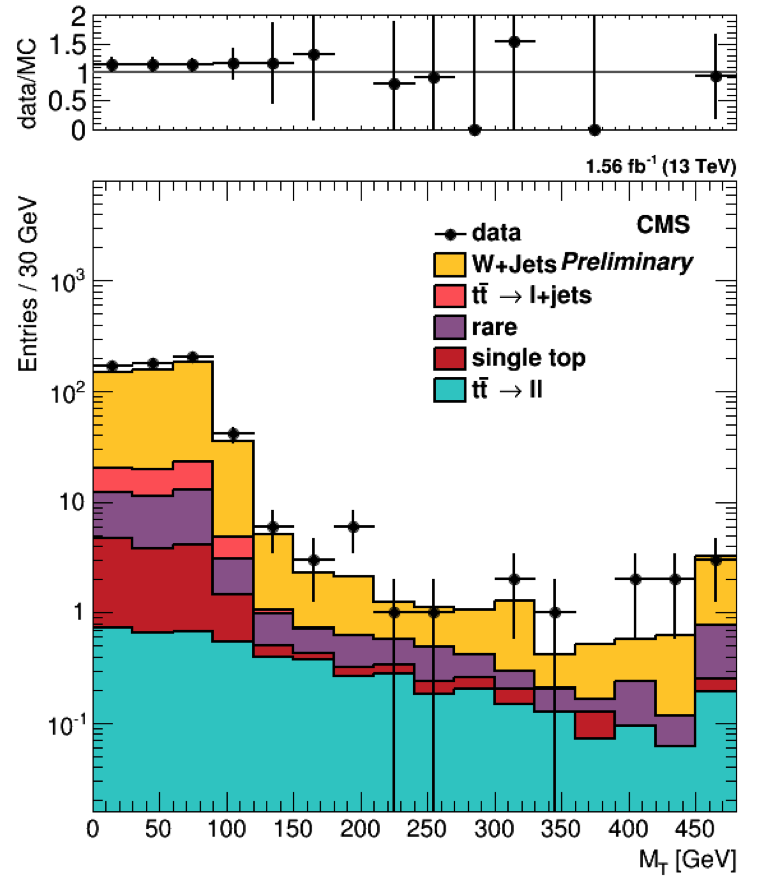
\includegraphics[width=0.44\textwidth]{Figures/bkg1lep/MTDist_3jets.png}
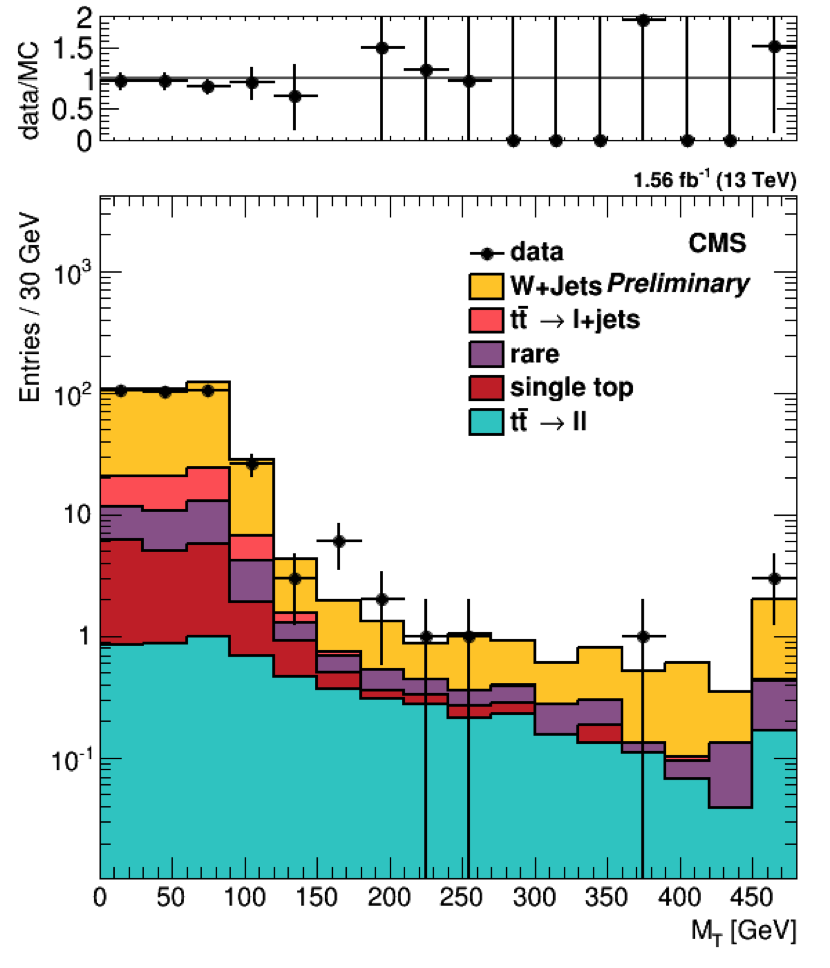
\includegraphics[width=0.44\textwidth]{Figures/bkg1lep/MTDist_4jets.png}
\caption{\label{fig:MT} Distribution of \MT for 3 and $\ge$ 4 jets 0b CRs.}
\end{figure}

The full MT distribution for the 0-btag CR is shown on Figure~\ref{fig:MT}.  There is good agreement between data and MC in both the peak region 
and the tail of the MT spectrum.  For the W+Jets, only the MT$>150$ \GeV region is used, to coincide with the requirement in the signal regions.  
The summary of yields for the CRs is shown on Table~\ref{tab:0b_CR:yields}.  All other 1-lepton background not from top decays will also be 
included in this estimate.  
%
As can be seen from Table~\ref{tab:0b_CR:yields},
there is close to 30\% contamination from dilepton and Z$\rightarrow\nu\nu$ backgrounds in these W+Jets CRs that needs to be subtracted.  
A 50$\%$ systematic uncertainty is assigned to this subtraction when calculating the  $N^{data,WJets}_{CR,0-btag}$.  

\begin{table}
\begin{center}
\small
\caption{\label{tab:0b_CR:yields} high $\Delta$M, 0b CR}
\resizebox{\textwidth}{!}{\begin{tabular}{|c|c|c|}\hline
  &==3 jets  & $\ge$ 4 jets  \\
 &MET $>$ 250&MET $>$ 250\\
\hline
1lep (not from top) $\pm \sigma^{MC}_{stat} $& 16.16$\pm$1.28 & 11.20$\pm$0.87\\
1lep (from top)$ \pm \sigma^{MC}_{stat} \pm \sigma^{MC}_{50\%syst} $& 0.08$\pm$0.03$\pm$0.04 & 0.39$\pm$0.08$\pm$0.19\\
$\ge$ 2lep (lost lep) $ \pm \sigma^{MC}_{stat} \pm \sigma^{MC}_{50\%syst} $  & 4.23$\pm$0.63$\pm$1.39 & 3.53$\pm$0.23$\pm$1.46\\
Z$\rightarrow\nu\nu  \pm \sigma^{MC}_{stat} \pm \sigma^{MC}_{50\%syst} $  & 3.74$\pm$0.15$\pm$1.69 & 1.99$\pm$0.11$\pm$0.84\\
Total BGs $ \pm \sigma^{MC}_{stat} \pm \sigma^{NonWJets MC}_{50\%syst} $ & 24.20$\pm$1.44$\pm$2.18 & 17.11$\pm$0.91$\pm$1.69\\
\hline
Data $\pm \sigma^{Data}_{stat}$ & 24.00$\pm$4.90 & 18.00$\pm$4.24\\
\hline
Data/MC  $\pm \sigma_{stat} \pm \sigma_{sys}$& 0.99$\pm$0.21$\pm$0.09 & 1.05$\pm$0.25$\pm$0.10\\
\hline
WJets purity $\pm \sigma_{stat} \pm \sigma_{sys}$ & 0.67$\pm$0.07$\pm$0.06 & 0.65$\pm$0.06$\pm$0.06\\
&&\\
N$^{data,WJets}_{0bCR}$: (1lep not from top) &15.96$\pm$4.90$\pm$0.65$\pm$2.19 & 12.09$\pm$4.24$\pm$0.27$\pm$1.70\\
&&\\
$\pm \sigma^{data}_{stat} \pm \sigma^{MC}_{stat} \pm \sigma^{MC}_{50\% syst}$&&\\\hline
\end{tabular}}
\end{center}
\end{table}

The final WJets estimates are shown in Table~\ref{tab:WJetsEstimate}.
\begin{table}
\begin{center}
\caption{\label{tab:WJetsEstimate}Values used for WJets Estimate with BTag SFs applied}
\resizebox{\textwidth}{!}{\begin{tabular}{|c|c|ccc|}\hline
\hline
  &==3 jets  && $\ge$ 4 jets &\\
 &MET $>$ 250& & MET $>$ 250&\\
 \hline
&&&&\\
N$^{data,WJets}_{0bCR2}$: (1lep not from top) &15.96 & & 12.09&\\
&&&&\\
$\pm \sigma^{data}_{stat} \pm \sigma^{MC}_{stat} \pm \sigma^{MC}_{50\% syst}$&$\pm$4.90$\pm$0.65$\pm$2.19&&$\pm$4.24$\pm$0.27$\pm$1.70&\\
\hline
&&&&\\
\hline
 &==3 jets  & $\ge$ 4 jets &$\ge$ 4 jets & $\ge$ 4 jets\\
 &MET $>$ 350&250 $<$ MET $<$ 350&350 $<$ MET $<$ 450&MET $>$ 450\\
 \hline
 &&&&\\
TF$_{MET}\pm \sigma^{MC}_{stat} $ & 0.37 $\pm$ 0.049 & 0.55 $\pm$ 0.073 & 0.25 $\pm$ 0.045 & 0.20 $\pm$ 0.033\\
&&&&\\
\hline
&&&&\\
TF$_{btags} \pm \sigma^{MC}_{stat}$& 0.18 $\pm$ 0.074 & 0.15 $\pm$ 0.032 & 0.29 $\pm$ 0.10 & 0.40 $\pm$ 0.19\\
&&&&\\
\hline
&&&&\\
WJets in SR & 1.06 & 0.96  & 0.86 & 0.98 \\
$\pm \sigma^{data}_{stat} \pm \sigma^{MC}_{stat} \pm \sigma^{MC}_{50\% syst}$  & $\pm$ 0.32 $\pm$ 0.43 $\pm$ 0.14 &  $\pm$ 0.34 $\pm$ 0.201 $\pm$ 0.13 &  $\pm$ 0.30 $\pm$ 0.28 $\pm$ 0.12 & $\pm$ 0.34 $\pm$ 0.45 $\pm$ 0.14 \\
&&&&\\
\hline
\end{tabular}}
\end{center}
\end{table}


\subsubsection{Systematic Uncertainties}
\label{subsec:bkg1l:sys}
The non-negligible systematic uncertainties affecting this background estimation are:
\begin{itemize}
  \item Data and MC statisitics - the largest uncertainty in the estimation is from the statistical uncertainty of the observed data yields in the CRs.
  \item W+b cross section - as we extrapolate in b-tagging using MC, we allow for a 50\% variation in the  W+b(b-bar) cross section.
  \item bTagging effiency and mistag rate - using SFs provided by the BTV POG.  Estimated by event reweighting using scale factors and MC b-tagging efficiencies %(Method 1a: https://twiki.cern.ch/twiki/bin/viewauth/CMS/BTagSFMethods#1a_Event_reweighting_using_scale)
  \item PDF - account for NNPDF3.0LO PDF variations.  Uncertainty is the standard deviatio of the average PDF variation.
  \item $Q^{2}$ - the largest two variations in renormalization and factorization scale,  $[\mu_{R}=2, \mu_{F}=2]  and [\mu_{R}=0.5, \mu_{F}=0.5]$,are considered 
  \item JES - the jet energy scale is varied, to account for diffences in jet acceptance. %as well as its effects on the calculation of t1 pfmet
  \item \MET resolution - a dedicated study described in Section~\ref{subsec:bkg1l:metResWithPhotons} is used to estimate uncertainties 
due to ``bin migration'' due to differences in the detailed shape of the \MET resolution function between data and MC. 
\end{itemize}
Table ~\ref{tab:1lepsysbtag} summarize the systematic uncertainties on the b-tag TF used to obtain the yield for each of the Signal Regions.  Table ~\ref{tab:1lepsys} shows the same for the \MET TF used to extrapolate in \MET.
\begin{table}
\begin{center}
\caption{\label{tab:1lepsysbtag}Systematic uncertainty on the b-tag TF}
\resizebox{\textwidth}{!}{\begin{tabular}{|c|c|ccc|}\hline
\hline
 &==3 jets  & $\ge$ 4 jets &$\ge$ 4 jets & $\ge$ 4 jets\\
 &MET $>$ 350&250 $<$ MET $<$ 350&350 $<$ MET $<$ 450&MET $>$ 450\\ 
\hline
Data Statistics&30$\%$&35$\%$&35$\%$&35$\%$\\
MC Statistics&41$\%$& 21 $\%$&32 $\%$&47.5$\%$\\
W+b xsec& 11$\%$ & 1$\%$ & 6$\%$ &7$\%$ \\
bTagging effiency and mistag rate&12$\%$ & 11$\%$ & 12$\%$ &12$\%$ \\
PDF&3$\%$ & 1$\%$ & 2$\%$ &5$\%$ \\
$Q^{2}$ &2$\%$ & 4.5$\%$ & 3$\%$ &4$\%$ \\
JES&11$\%$ & 11$\%$ & 5$\%$ &10$\%$ \\
Contamination in CR &14$\%$ &14$\%$ &14$\%$ & 14$\%$ \\
\hline
\end{tabular}}
\end{center}
\end{table}

\begin{table}
\begin{center}
\caption{\label{tab:1lepsys}Systematic uncertainty on the \MET TF}
\resizebox{\textwidth}{!}{\begin{tabular}{|c|c|ccc|}\hline
\hline
 &==3 jets  & $\ge$ 4 jets &$\ge$ 4 jets & $\ge$ 4 jets\\
 &MET $>$ 350&250 $<$ MET $<$ 350&350 $<$ MET $<$ 450&MET $>$ 450\\ 
\hline
MC Statistics&13$\%$&13$\%$&18$\%$&17$\%$\\
W+b xsec&1.4$\%$&0.3$\%$&0.4$\%$&0.4$\%$\\
bTagging effiency and mistag rate&1.$\%$&1.$\%$&1.$\%$&1.$\%$\\
PDF&1$\%$&1$\%$&1$\%$&1$\%$\\
$Q^{2}$ &2$\%$&1$\%$&1$\%$&1$\%$\\
JES&1$\%$&5$\%$&5$\%$&7$\%$\\
\MET resolution $\%$ & & & \\
\hline
\end{tabular}}
\end{center}
\end{table}

\subsubsection{Systematics due to differences in \MET resolution function between data and MC}
\label{subsec:bkg1l:metResWithPhotons}

{\bf fkw comment: here we describe HJ's study with photons}

\subsubsection{Summary of One Lepton background estimate}
\label{sec:bkg1l:summary}

{\bf fkw comment: we still need to add in the pieces that come from MC straight up, and add it to the data derived stuff.}
